\documentclass[aspectratio=169]{beamer}
\usepackage[utf8]{inputenc}
%\usepackage[authordate,backend=biber,natbib]{biblatex-chicago}
%\usepackage{booktabs}
%\addbibresource{growthreferences.bib}

%\usepackage{utopia} %font utopia imported

\usetheme{Madrid}
\usecolortheme{beaver}

%------------------------------------------------------------
%This block of code defines the information to appear in the
%Title page
\title[Bowen, Leamer, and Sveikauskas (1987)] %optional
{Multicountry, Multifactor Tests of the Factor Abundance Theory}

\subtitle{Harry Bowen, Edward Leamer, and Leo Sveikauskas, \emph{The American Economic Review}, 1987}

\author [Hauk] % (optional)
{William~R.~Hauk,~Jr.} %\inst{1} %\and J.~Doe\inst{2}} 

\institute[UofSC] % (optional)
{
  %\inst{1}%
  Darla Moore School of Business\\
  University of South Carolina
  %\and
  %\inst{2}%
  %Faculty of Chemistry\\
  %Very Famous University
}

\date[ECON 860, Fall 2021] % (optional)
{ECON 860 -- International Trade Theory\\Fall 2021}

\logo{
\includegraphics[height=1cm]{UofSC_Monogram_Stack_CMYK_G.jpg}}

%End of title page configuration block

%---------------------------------------------------------

\AtBeginSection[]
{
  \begin{frame}
    \frametitle{Table of Contents}
    \tableofcontents[currentsection]
  \end{frame}
}

%------------------------------------------------------------

\begin{document}

%The next statement creates the title page.
\frame{\titlepage}

%---------------------------------------------------------
\section{Introduction}
\begin{frame}{Motivation}

Paper claims that most tests of the Heckscher-Ohlin Model are lacking on two counts:

\begin{itemize}
    \item<1-> The original $ 2 \times 2 $  H-O model doesn’t generalize in an unambiguous fashion to a multi-factor, multi-good world.  
    \item<2-> H-O theorem describes a relationship between three separate phenomena: trade, factor input requirements, and factor endowments.  Most tests before BLS only used data on 2 out of these 3 variables.
\end{itemize}
    
\end{frame}

%---------------------------------------------------------

\begin{frame}{Leontief's Paradox}

Leontief (1953) provides the first test of the Heckscher-Ohlin Theorem.

\begin{itemize}
    \item<1-> He finds that factor requirements of U.S. imports are more labor-intensive than U.S. exports.
    \item<2-> He only uses capital and labor as factors, which Leamer (1980) shows does not generalize to a multi-factor world.
    \item<3-> Also, he only has data on factor requirements, not factor endowments.
\end{itemize}
    
\end{frame}

%--------------------------------------------------------------

\begin{frame}{Regression Studies \# 1}

One strand of literature tries to test the H-O Theorem by regressing trade of various commodities on their factor input requirements for a country.

\begin{itemize}
    \item<1-> Sign of regression coefficient should reveal country’s abundance in that factor. (E.g. Baldwin (1971), Branson and Monoyios (1977), Harkness (1978, 1983), Stern and Maskus (1981))
    \item<2-> Problem is that there is no factor endowment data to check predictions against.  Bowen and Leamer (1981) show that coefficients might be misleading.
\end{itemize}

\end{frame}

%--------------------------------------------------------------

\begin{frame}{Regression Studies \# 2}

Another strand regresses net exports for a single commodity on factor endowments for different countries.

\begin{itemize}
    \item<1-> Tests a weakened version of H-O Theorem that says that trade can be explained somehow by factor endowments, but does not make an explicit link with factor requirements. (E.g. Bowen (1983), Chenery and Syrquin (1975), Leamer (1974, 1984))
\end{itemize}
    
\end{frame}

%--------------------------------------------------------------

\begin{frame}{Purpose of This Paper}

\begin{itemize}
    \item<1-> This paper computes the amount of 12 factors embodied in the net exports of 27 countries in 1967, using a U.S. input-output matrix for 1966.
    \item<2-> Analysis has data on all three elements:  trade flows, factor requirements, and factor endowments.
    \item<3-> Results are generally not very supportive of the Heckscher-Ohlin Model.
\end{itemize}
    
\end{frame}

%---------------------------------------------------------------

\section{Heckscher-Ohlin-Vanek Model}

%---------------------------------------------------------------

\begin{frame}{Vanek (1967) Model}

Vanek (1967) creates an extension of the Heckscher-Ohlin Model (henceforth, HOV Model) for an arbitrarily large number of $ M $ factors, $ N $ goods, and $ C $ countries.

\begin{itemize}
    \item<1-> Start with country $ i $'s trade balance:
    \begin{equation*}
        \mathbf{T}^i = \mathbf{Y}^i - \mathbf{D}^i
    \end{equation*}
    where each element is an $ N \times 1 $ vector of goods -- $ \mathbf{T}^i $ is a vector of net exports (each element could be positive or negative), $ \mathbf{Y}^i $ is a vector of production, and $ \mathbf{D}^i $ is a vector of consumption.
    \item<2-> Pre-multiply both sides by an $ M \times N $ input-output matrix $ \mathbf{A} $:
    \begin{equation}
        \mathbf{AT}^i = \mathbf{AY}^i - \mathbf{AD}^i
        \label{eq:factorcontenttrade}
    \end{equation}
    Note that $ \mathbf{A} $ does not have a superscript.  This is because we assume identical production technologies across all countries.
\end{itemize}
    
\end{frame}

%---------------------------------------------------------------

\begin{frame}{HOV Model \# 2}

\begin{itemize}
    \item<1-> Define $ \mathbf{F}^i = \mathbf{AT}^i $ as country $ i $’s “factor content of trade” – that is, the  $ M \times 1 $ vector of factor inputs embedded in the country’s net trade of goods (each element could be either positive or negative).
    \item<2-> Due to the assumption of full-employment in the H-O model, we can write $ \mathbf{AY}^i = \mathbf{V}^i $, where $ \mathbf{V}^i $ is the $ M \times 1 $ vector of country $ i $’s factor endowments.
    \item<3-> If world supply equals world demand, then $ \sum_{i=1}^{C} {\mathbf{D}^i} = \mathbf{Y}^w $.  If utility functions are homothetic across countries (as is assumed in the H-O model), then $ \mathbf{D}^i = s^{i} \mathbf{Y}^w $, where $ s^i $ is country $ i $'s share of world income.
\end{itemize}
    
\end{frame}

%---------------------------------------------------------------

\begin{frame}{HOV Model \# 3}

\begin{itemize}
    \item<1-> Assuming full employment of factors across countries gives us $ \mathbf{AD^{i}} = s^{i} \mathbf{AY^{w}}= s^{i} \mathbf{V^{w}} $.
    \item<2-> Combining all of the above, we can then rewrite equation (\ref{eq:factorcontenttrade}) as:
    \begin{equation}
        \mathbf{F^{i}} = \mathbf{V^{i}} - s^{i} \mathbf{V^{w}}
        \label{eq:HOVequation}
    \end{equation}
    That is, the factor content of country $ i $’s trade will be equal to the difference between country $ i $’s factor endowment and the world factor endowment multiplied by country $ i $’s share of world income.
    \item<3-> This equation forms the basis of the empirical tests in BLS.
\end{itemize}
    
\end{frame}

%---------------------------------------------------------------

\section{Tests of Qualitative Hypotheses}

%---------------------------------------------------------------

\begin{frame}{Data}

Data come from the 367-element U.S. input-output table for 1967, and factor supply and trade data for 27 countries.

\begin{itemize}
    \item<1-> Factors looked at are: net capital stock, total labor, professional/technical workers, managerial workers, clerical workers, sales workers, service workers, agricultural workers, production workers, arable land, pasture land, and forest land.
    \item<2-> Trade data for each country’s trade is obtained at the 4 and 5-digit level of the Standard International Trade Classification (SITC) industry classification, and concorded to the U.S. input-output table.
\end{itemize}
    
\end{frame}

%---------------------------------------------------------------

\begin{frame}{Sign Test}

The first test that BLS try is a sign test:

\begin{itemize}
    \item<1-> The $ k $th element of equation (\ref{eq:HOVequation}) can be written as:
    \begin{equation*}
        \frac{F_{k}^{i} / V_{k}^{w}}{Y^{i} / Y^{w}} = \left[ \frac{V_{k}^{i} / V_{k}^{w}}{Y^{i} / Y^{w}} \right] - 1
    \end{equation*}
    (i.e. if the term in brackets on the right is greater than 1, then the country is abundant in the factor, and scarce if it is less than 1).
    \item<2-> The sign test checks to see if the sign on the left-hand side of the equation is the same as the sign on the right-hand side of the equation – i.e. if the country has a positive factor-content of trade for factor  $ k $, then the country should be abundant in factor $ k $, and conversely if the signs are negative.
\end{itemize}
    
\end{frame}

%---------------------------------------------------------------

\begin{frame}{Rank Test}

The other type of qualitative test used by BLS is a rank test:

\begin{itemize}
    \item<1-> The rank test checks if the relative factor content of trade reveals the relative abundance of resources, that is, if we have two factors $ k $ and  $ l $, then:
    \begin{equation*}
        \frac{F_{k}^{i} / V_{k}^{w}}{Y^{i} / Y^{w}} > \frac{F_{l}^{i} / V_{l}^{w}}{Y^{i} / Y^{w}} \Leftrightarrow  \frac{V_{k}^{i} / V_{k}^{w}}{Y^{i} / Y^{w}} > \frac{V_{l}^{i} / V_{l}^{w}}{Y^{i} / Y^{w}}
    \end{equation*}
    that is, if a country has a relatively higher factor content of trade for factor $ k $ than factor $ l $, then it should have a relatively higher factor endowment for factor $ k $ than factor $ l $, and vice versa.
\end{itemize}
    
\end{frame}

%---------------------------------------------------------------

\begin{frame}{Sign and Rank Test Results \#1}

Table 1 shows $ F_{k,i} / V_{k,w} $ for a number of countries and factors of production in 1966-67.  Note that, contrary to Leontief Paradox, U.S. seems to export capital services and import labor services.

\begin{figure}
    \centering
    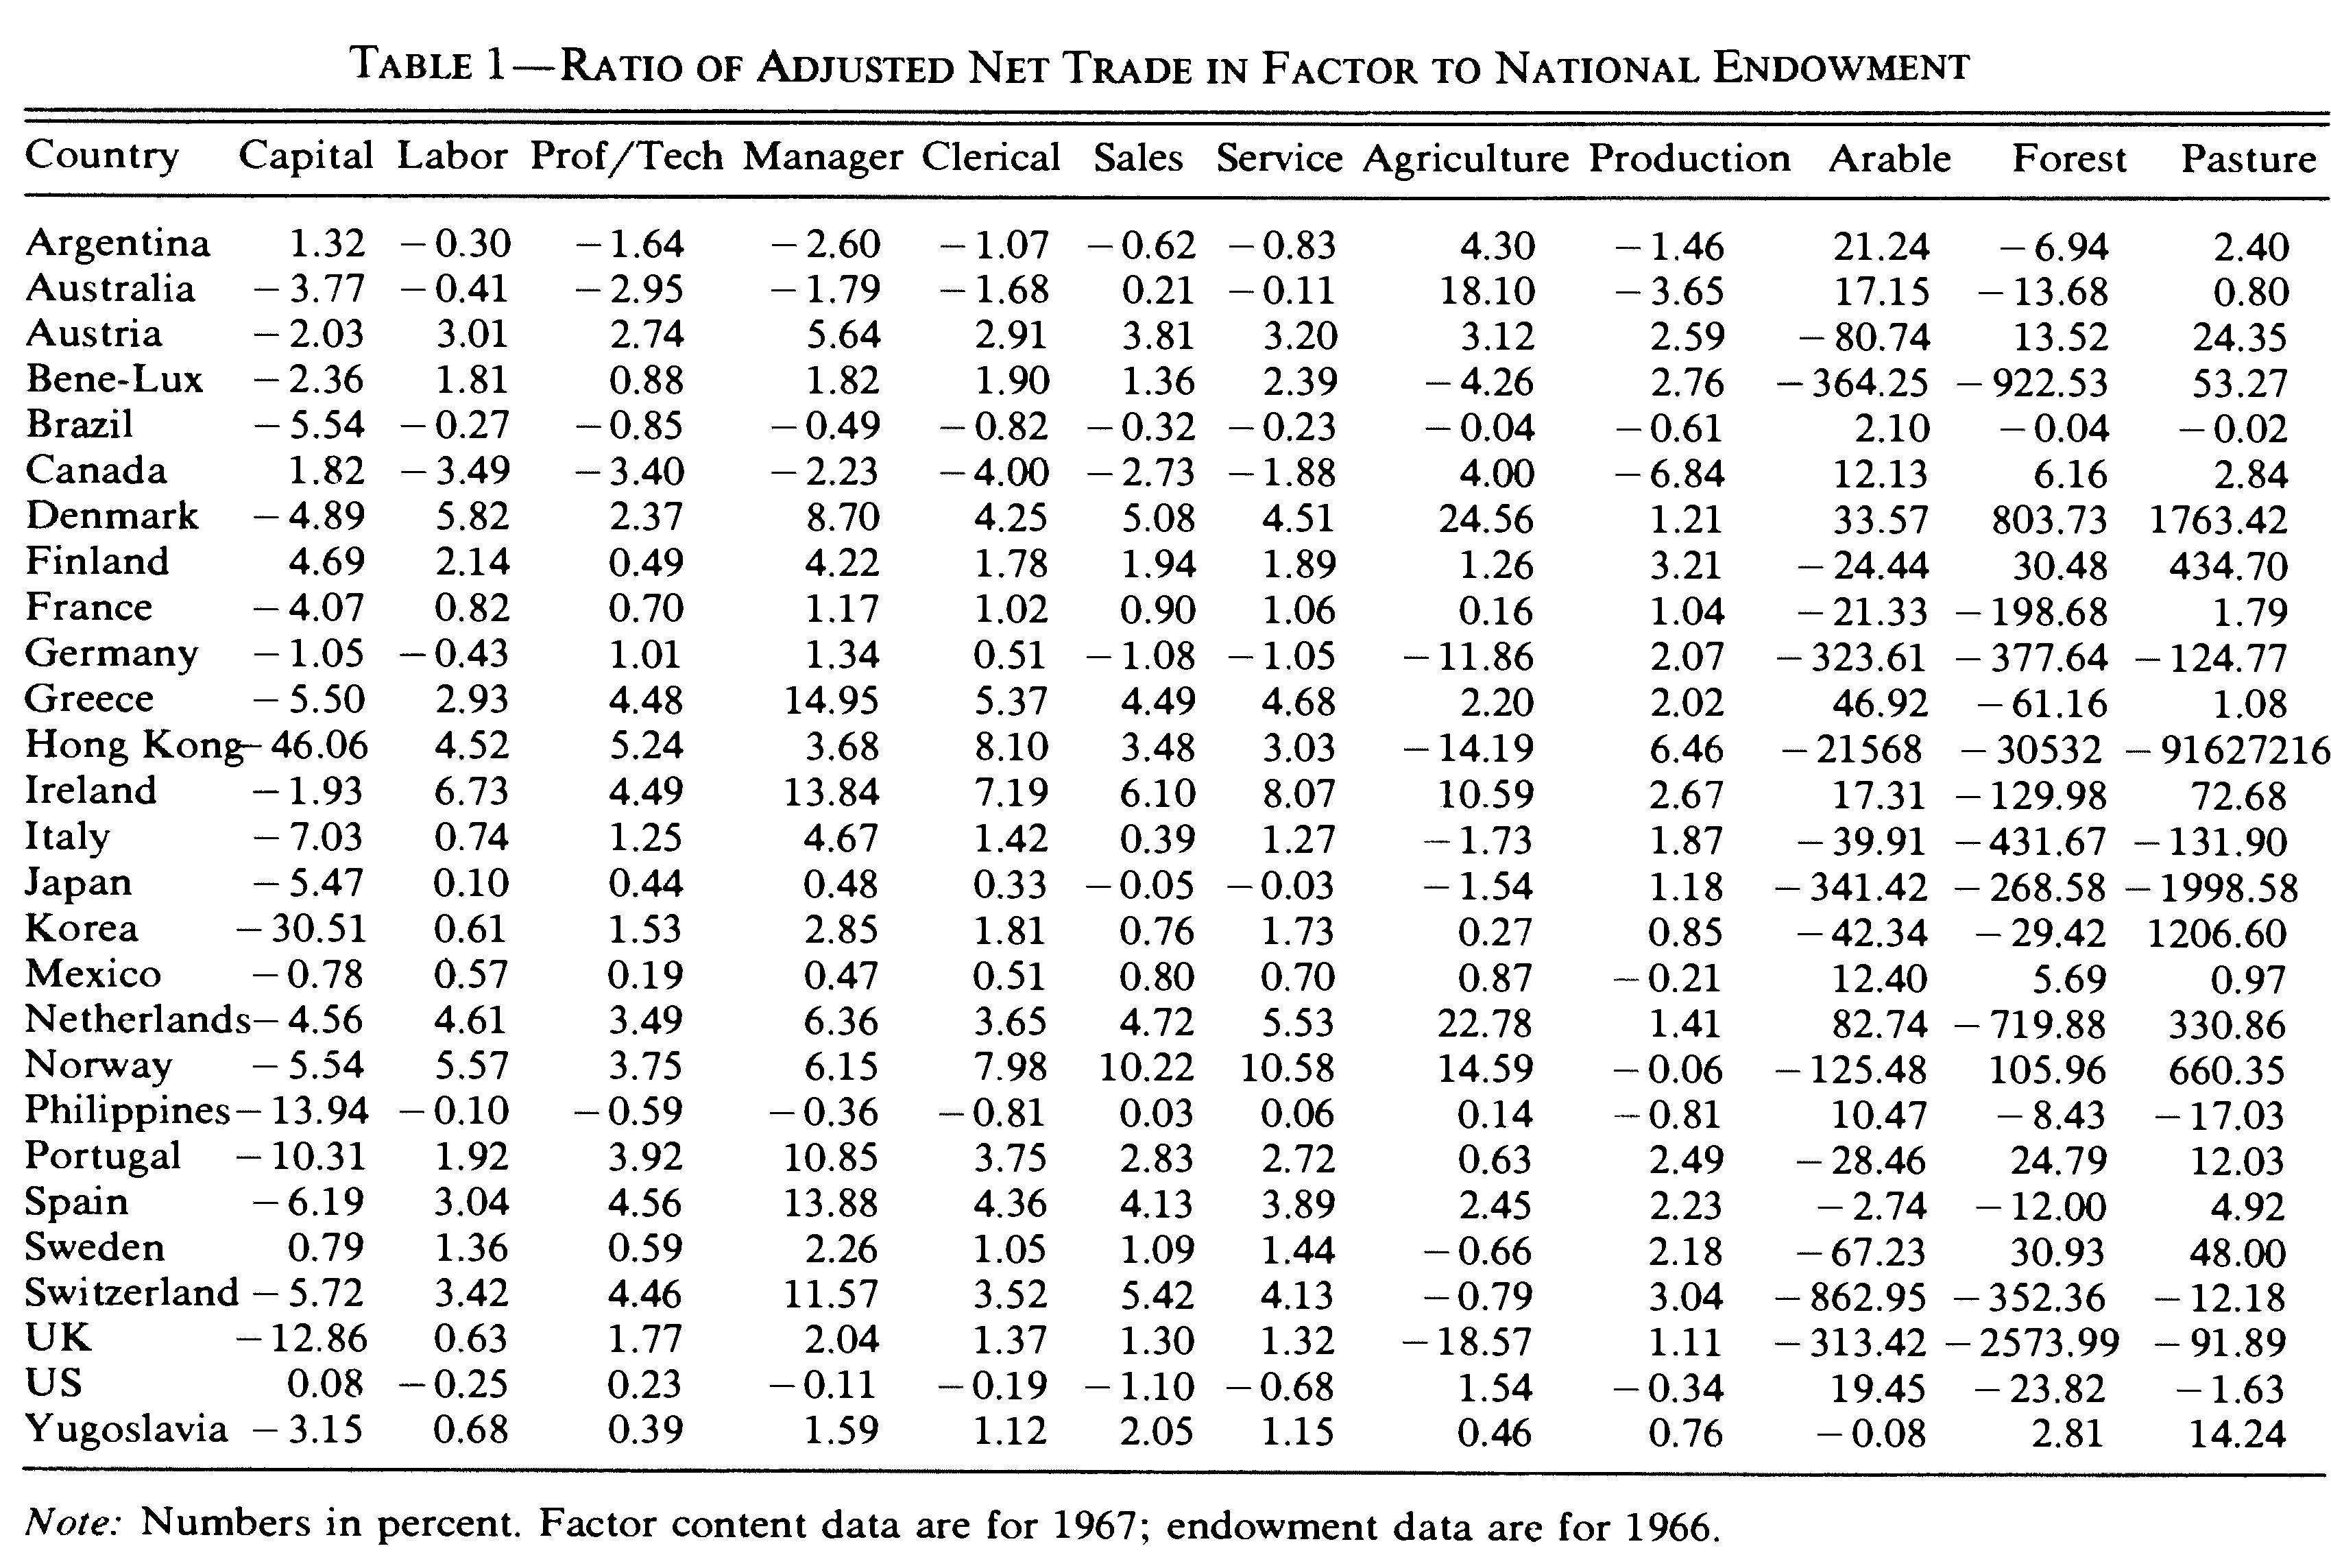
\includegraphics[scale = 0.57]{Table 1.png}
    \label{fig:Table1}
\end{figure}
    
\end{frame}

%---------------------------------------------------------------

\begin{frame}{Sign and Rank Test Results \#2}

Table 2 shows in the first column the proportion of ``correct” matches for signs by different factors across countries and the rank test in the second and third columns.

\begin{figure}
    \centering
    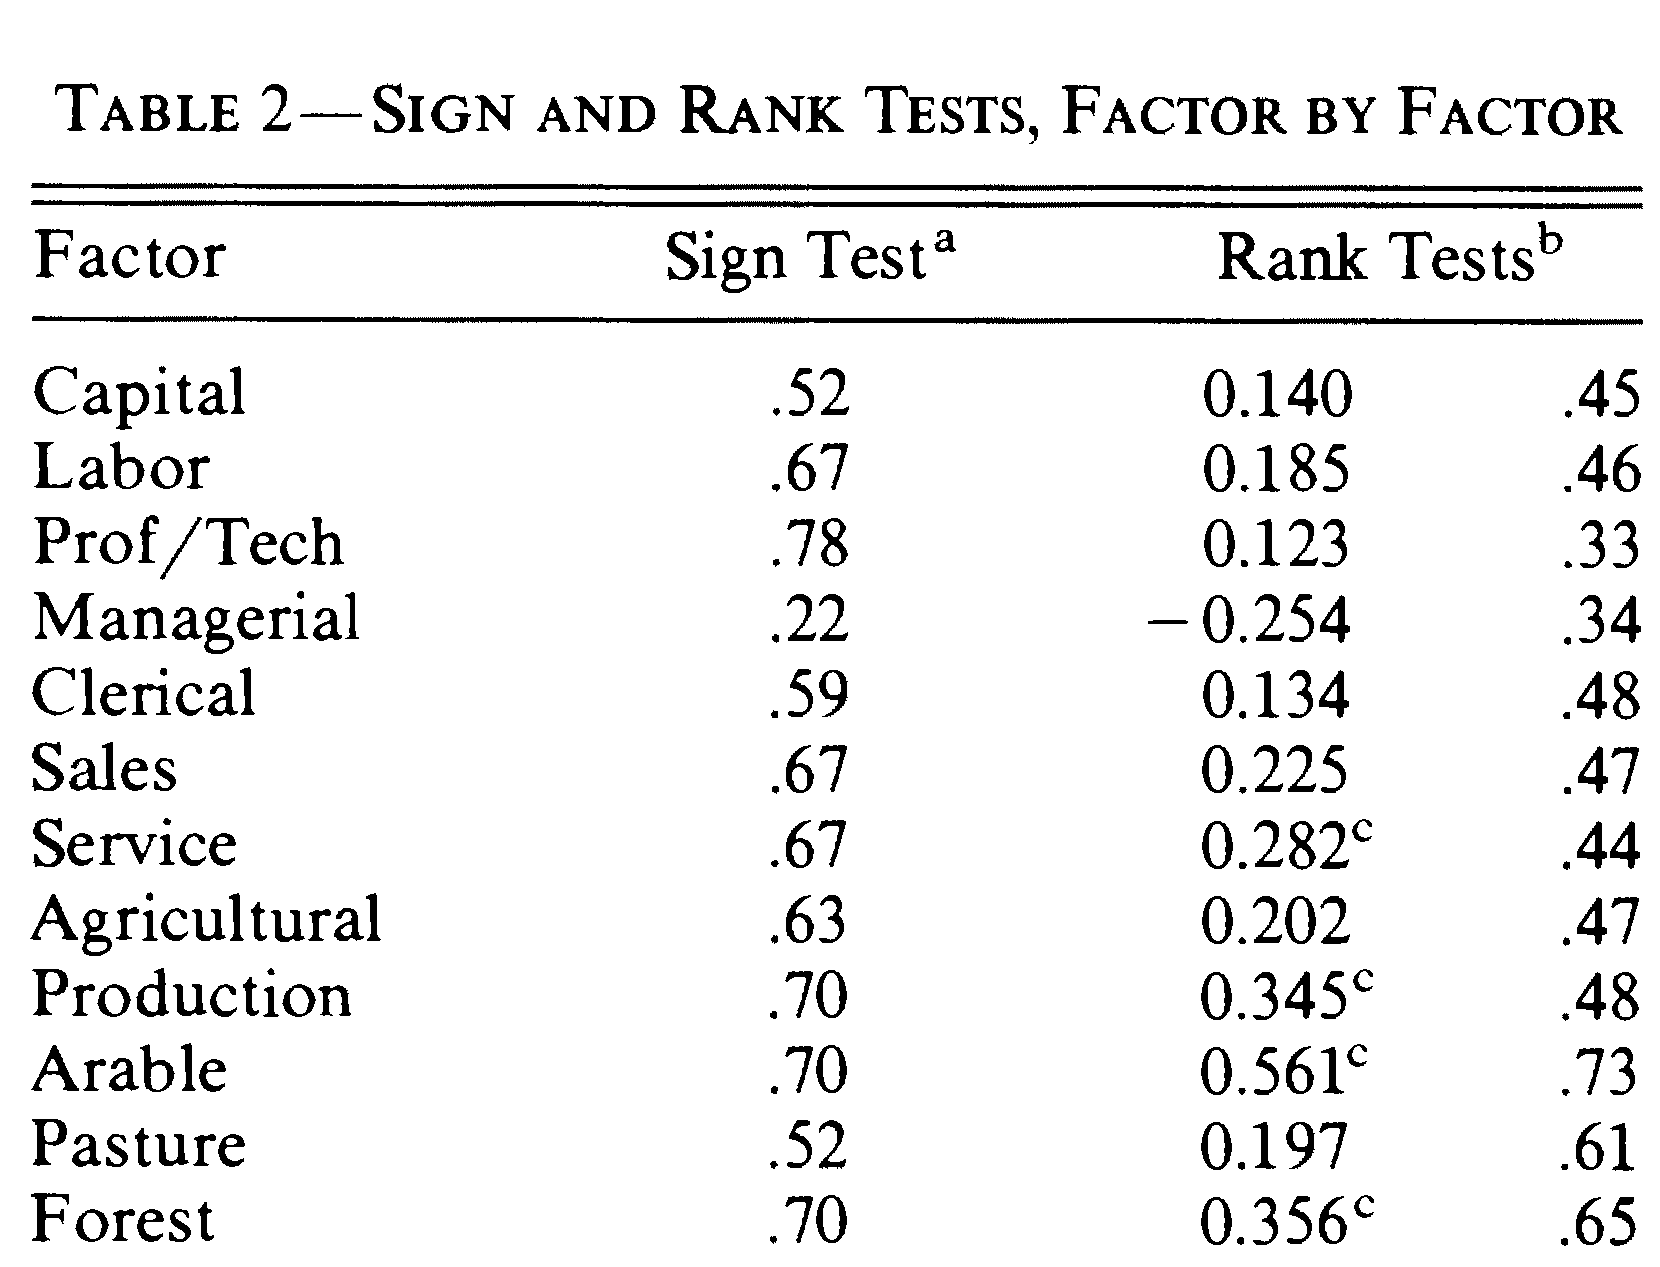
\includegraphics[scale = 1.1]{Table 2.png}
    \label{fig:Table2}
\end{figure}
    
\end{frame}

%---------------------------------------------------------------

\begin{frame}{Sign and Rank Test Results \#3}

\begin{itemize}
    \item<1-> Sign test exceeds $ 50\% $ for 11 of the 12 factors.  However, only 4 of the 12 are $ 70\% $ or higher, and only one, Arable Land, is significant at the $ 5\% $ level.
    \item<2-> Rank test is mixed.  11 of 12 Kendall rank correlation coefficients are positive, but only 4 of 12 are significant at the $ 5\% $ level.
\end{itemize}
    
\end{frame}

%---------------------------------------------------------------

\begin{frame}{Sign and Rank Test Results \#4}

Table 3 repeats the sign and rank test across factors by country.
 
\begin{figure}
    \centering
    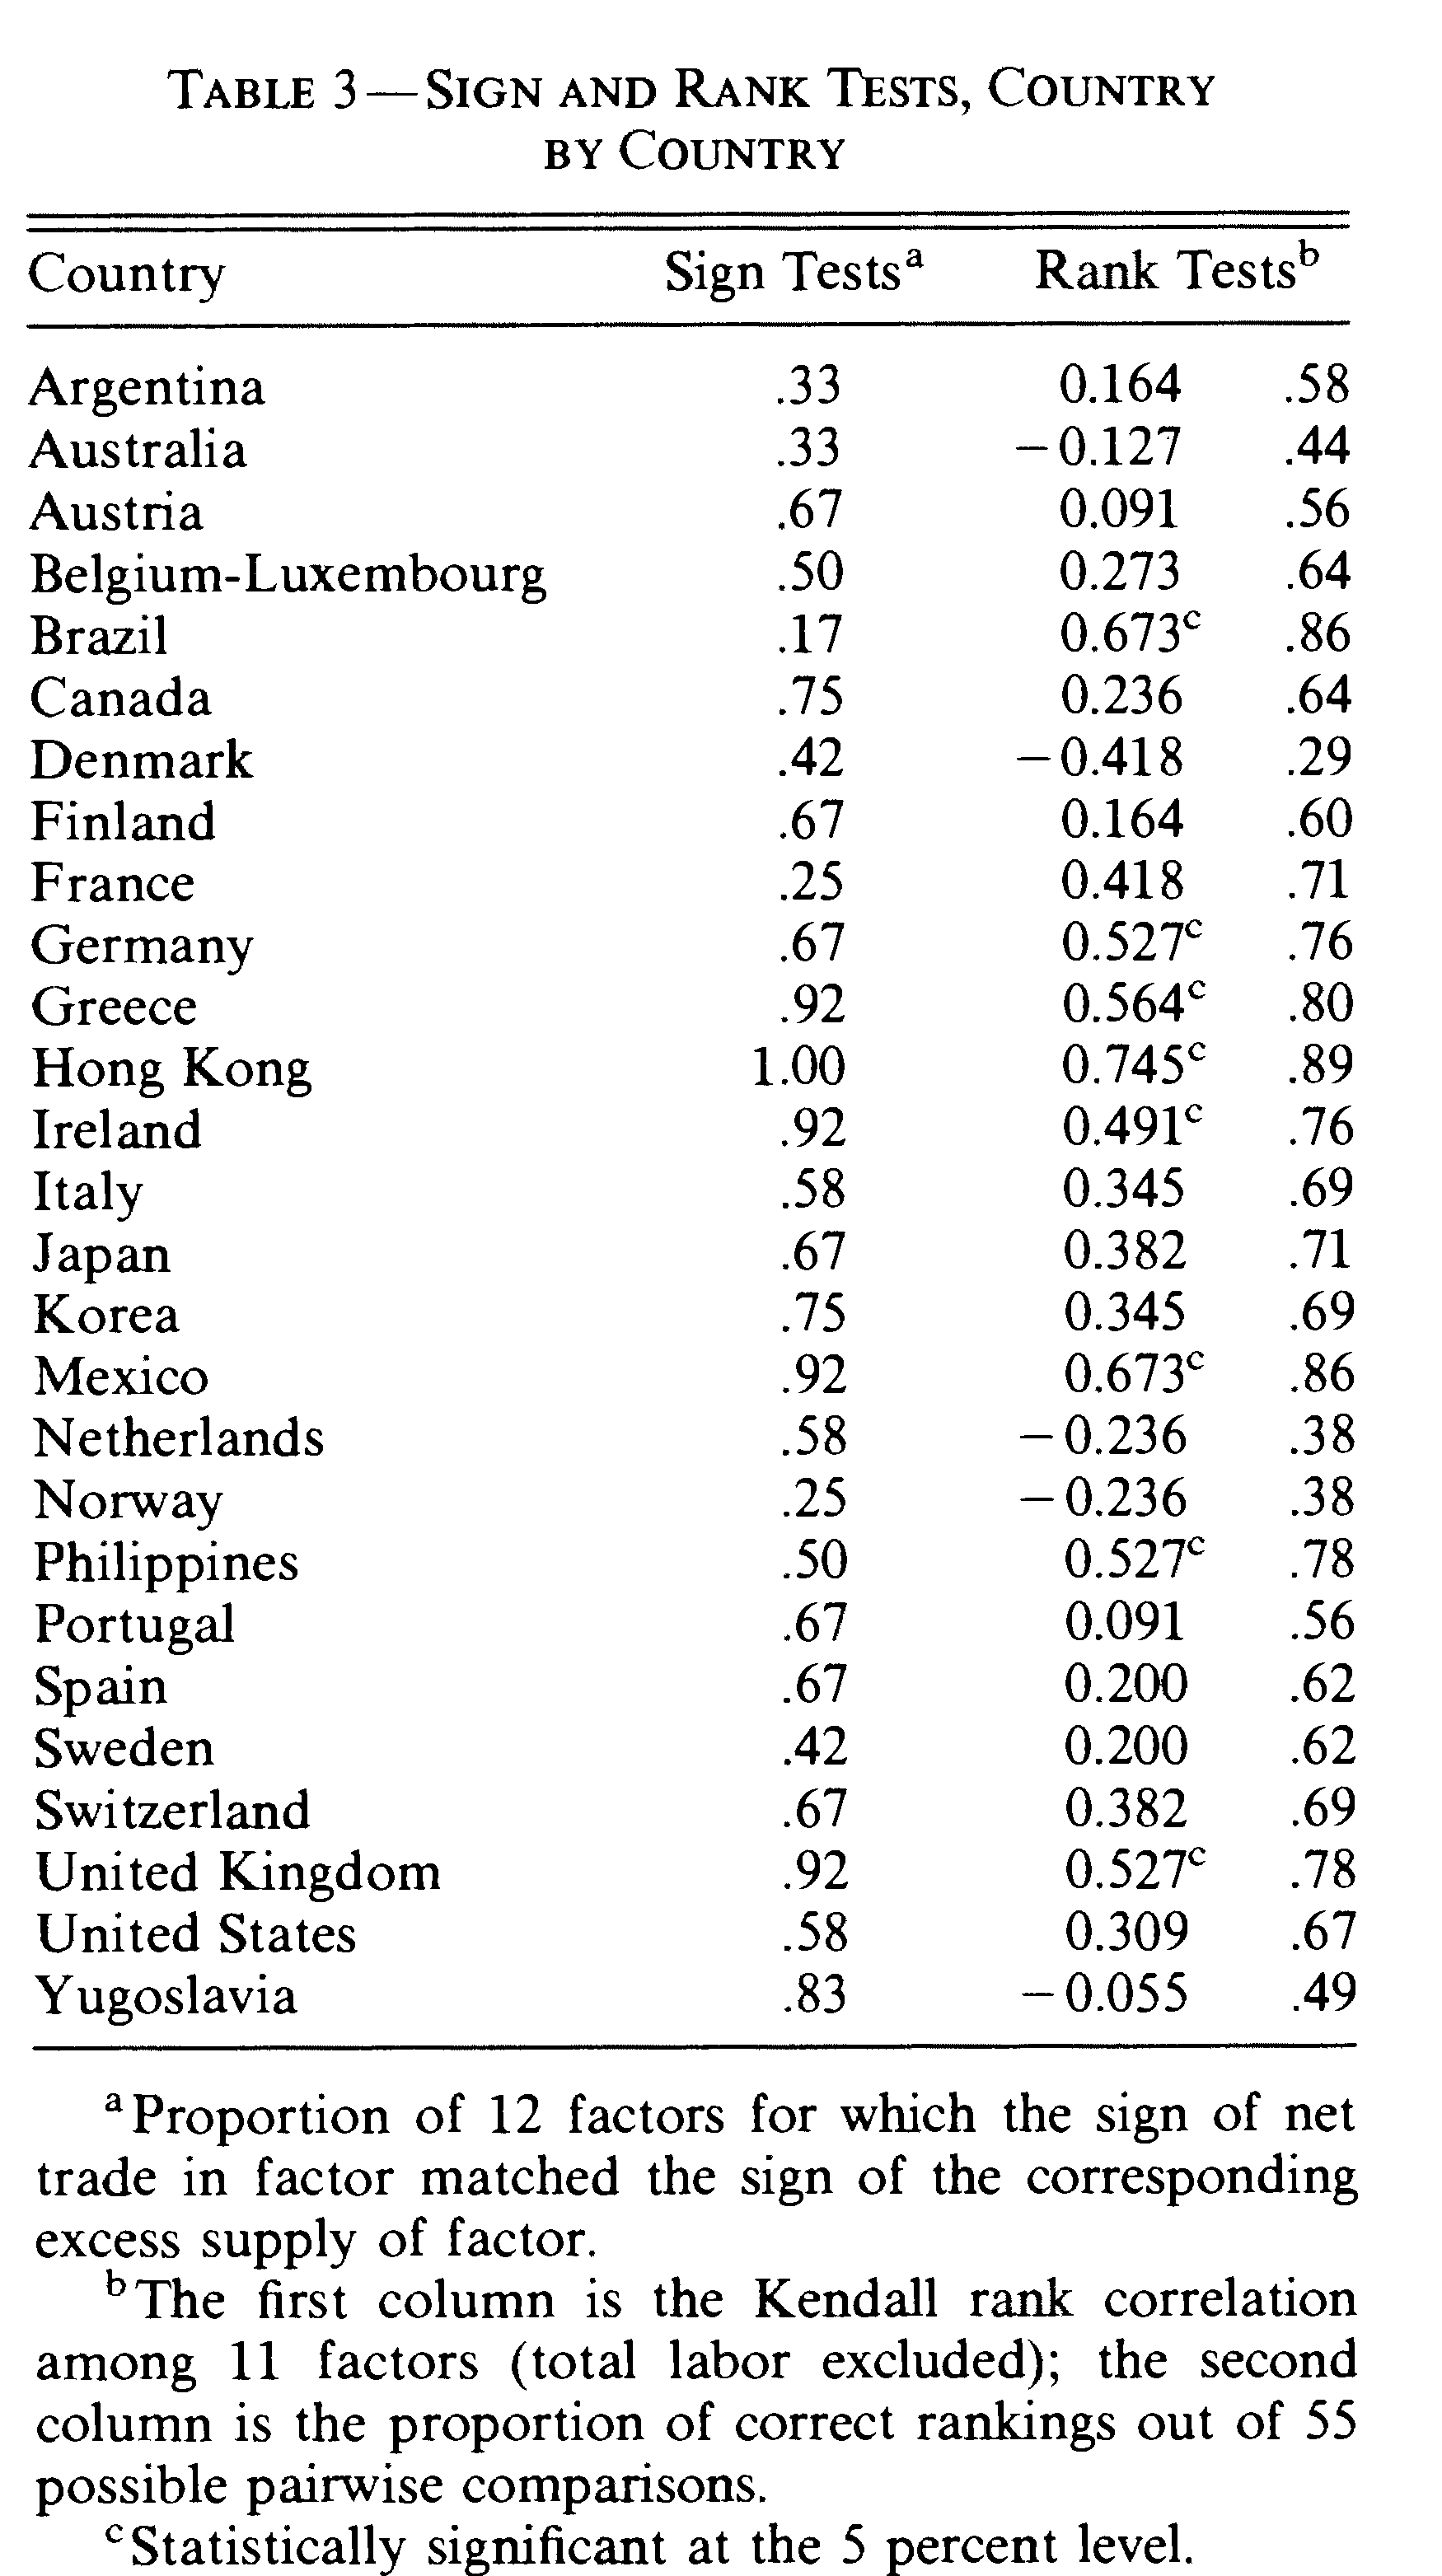
\includegraphics[scale = 0.5]{Table 3.png}
    \label{fig:Table3}
\end{figure} 
    
\end{frame}

%---------------------------------------------------------------

\begin{frame}{Sign and Rank Test Results \#5}

\begin{itemize}
    \item<1-> Sign test exceeds $ 50\% $ for only 18 of 27 countries, and $ 70\% $ for 8 of 27 countries.  Only significant at $ 5\% $ level for 4 of 27 countries (Greece, Ireland, Hong Kong, and the U.K.).
    \item<2-> For rank correlation, 5 of 27 countries have the wrong sign, only 8 countries have correct sign and significantly different from zero at the $ 5\% $ level.  Pairwise comparisons are greater than $ 50\% $ for 22 countries.
    \item<3-> Qualitative tests are generally not very supportive of the HOV model, but it is difficult to tell the reason why.
\end{itemize}
    
\end{frame}

%---------------------------------------------------------------

\section{Regression Tests of HOV Equations}

\subsection{Alternative Hypotheses}

%---------------------------------------------------------------

\begin{frame}{Alternative Hypothesis:  Homothetic Preferences}

H-O-V Model assumes homothetic (proportional) consumer preferences.  Relaxing all assumptions about consumption preferences would make the relation between trade and factor endowments completely indeterminate, but we can test a specific alternative.

\begin{itemize}
    \item<1-> Alternate Hypothesis (A2):  All individuals have identical preferences with linear Engel curves; and within each country, income is equally distributed.  Consumption of good $ j $ is:
    \begin{equation}
        C_{i,j} = \lambda_{j}L_{i} + \psi_{j}\left( \left( Y_{i} - B_{i} \right) - L_{i}y^{0} \right)
        \label{eq:hypothesisA2}
    \end{equation}
    \item<2-> Equation (\ref{eq:hypothesisA2}) implies that equation (\ref{eq:HOVequation}) can be rewritten as:
    \begin{equation*}
        \mathbf{F_{i}} = \mathbf{V_{i}} - \mathbf{\theta}L_{i} - \mathbf{\beta}\left( Y_{i} - B_{i} \right)
    \end{equation*}
    where our original assumption is nested within this specification if we restrict $ \mathbf{\theta} = 0 $ and $ \beta_k = V_{k,w} / Y_{w} $/
\end{itemize}
    
\end{frame}

%---------------------------------------------------------------

\begin{frame}{Alternative Hypothesis:  Measurement Error \#1}

We also assume that trade vectors and factor endowment vectors, which may be tricky to measure in practice, are not measured with error:

\begin{itemize}
    \item<1-> Alternative Hypothesis (M1):  The measurement of net trade vectors are measured with error, where the measured net trade differs from the true value by a constant plus a random error:
    \begin{equation*}
        \mathbf{T_{i}^{m}} = \omega + \mathbf{T_{i}} + \mathbf{T_{i}^{e}}
    \end{equation*}
    which, in turn, implies that the factor content of trade is:
    \begin{equation*}
         \begin{split}
            \mathbf{F_{i}^{m}} = \mathbf{AT_{i}^{m}} &= \mathbf{A}\omega + \mathbf{AT_{i}} + \mathbf{AT_{i}^{e}} \\ &= \alpha + \mathbf{F_{i}} + \mathbf{F_{i}^{e}}
        \end{split}
    \end{equation*}
   and our original assumption is nested in this specification by assuming that $ \alpha = 0 $.
\end{itemize}
    
\end{frame}

%---------------------------------------------------------------

\begin{frame}{Alternative Hypothesis:  Measurement Error \#2}

\begin{itemize}
    \item<1-> Alternative Hypothesis (M2):  The measurements of factor endowments are also imperfect, but in the following manner:
    \begin{equation*}
        V_{k,i} = \gamma_{k}V_{k,i}^{m}
    \end{equation*}
    where the original assumption is nested by assuming that $ \gamma_{k} = 1 $ for all $ k $.
\end{itemize}
    
\end{frame}

%---------------------------------------------------------------

\begin{frame}{Alternative Hypothesis:  Measurement Error \#3}

Measurement error may also affect the total world endowments, especially because we have incomplete coverage of countries.  This isn’t a big problem if the sum of endowments in our sample is roughly proportional to the world endowment, but we don’t know that it is.

\begin{itemize}
    \item<1-> Alternative Hypothesis (M3):  Assume that the calculated totals from the sample do not accurately represent the world totals so that:
    \begin{equation*}
        V_{k,w} = \sigma_{k,S}V_{k,S}
    \end{equation*}
    \begin{equation*}
        Y_{w} = \phi_{S}Y_{S}
    \end{equation*}
    where $ S $ is the total of the countries in the sample, and $ \phi $ and $ \sigma $ are unknown elements.  The original assumption is nested by assuming that $ \sigma = 1 $ and $\phi = 1 $ for all $ k $. 
\end{itemize}
    
\end{frame}

%---------------------------------------------------------------

\begin{frame}{Modified Regression Equation}

If we combine all of the alternative assumptions above, we can write a regression equation of the following form:

\begin{equation}
    F_{k,i} = \alpha_{k} + \gamma_{k}V_{k,i} - \theta_{k}L_{i} - \beta_{k}\left( Y_{i} - B_{i} \right) + F_{i,k}^{e}
    \label{eq:modifiedequation1}
\end{equation}

where all of the variables are the measured amounts.
    
\end{frame}

%---------------------------------------------------------------

\begin{frame}{Technological Heterogeneity}

We have assumed (along with the H-O-V Model) that all countries use the same technology as the U.S..  Relax this assumption slightly by allowing a proportional deviation from the U.S. input-output matrix.

\begin{itemize}
    \item<1-> Alternative Hypothesis (A3):  We measure other countries’ input-output matrix as proportional to the U.S. matrix:
    \begin{equation*}
        \mathbf{A_{US}} = \delta_{i} \mathbf{A_{i}}
    \end{equation*}
    where $ \delta_{i} > 0 $ and $ \delta_{US} = 1 $.
    \item<2-> Under hypothesis (A3), $ \theta_{k} $ becomes $ \theta_{k} / \delta_{i} $, $ \beta_{k} $ becomes $ \beta_{k} / \delta_{i} $, and $ F_{k,i} $ becomes $ F_{k,i}^{US} / \delta_{i} $ where $ F_{k,i}^{US} $ is country $ i $'s factor content of trade for factor $ k $ using the U.S. input-output matrix.
\end{itemize}
    
\end{frame}

%---------------------------------------------------------------

\begin{frame}{Regression Equation}

If we substitute the values generated by hypothesis (A3) into equation (\ref{eq:modifiedequation1}), we get:

\begin{equation*}
    \frac{F_{k,i}^{US}}{\delta_{i}} = \frac{\alpha_{k}}{\delta_{i}} + \gamma_{k}V_{k,i} - \frac{\theta_{k}}{\delta_{i}}L_{i} - \frac{\beta_{k}}{\delta_{i}}\left( Y_{i} - B_{i} \right) + \frac{F_{k,i}^{e}}{\delta_{i}}
\end{equation*}

And multiplying through by $ \delta_{i} $, we get:

\begin{equation}
    F_{k,i}^{US} = \alpha_{k} + \left( \delta_{i} \gamma_{k} \right)V_{k,i} - \theta_{k}L_{i} - \beta_{k}\left( Y_{i} - B_{i} \right) + F_{k,i}^{e}
    \label{eq:generalregressionmodel}
\end{equation}
    
\end{frame}

%---------------------------------------------------------------

\begin{frame}{Parameter Restrictions}

We can turn different assumptions on and off via parameter restrictions, which are noted in Table 4:

\begin{figure}
    \centering
    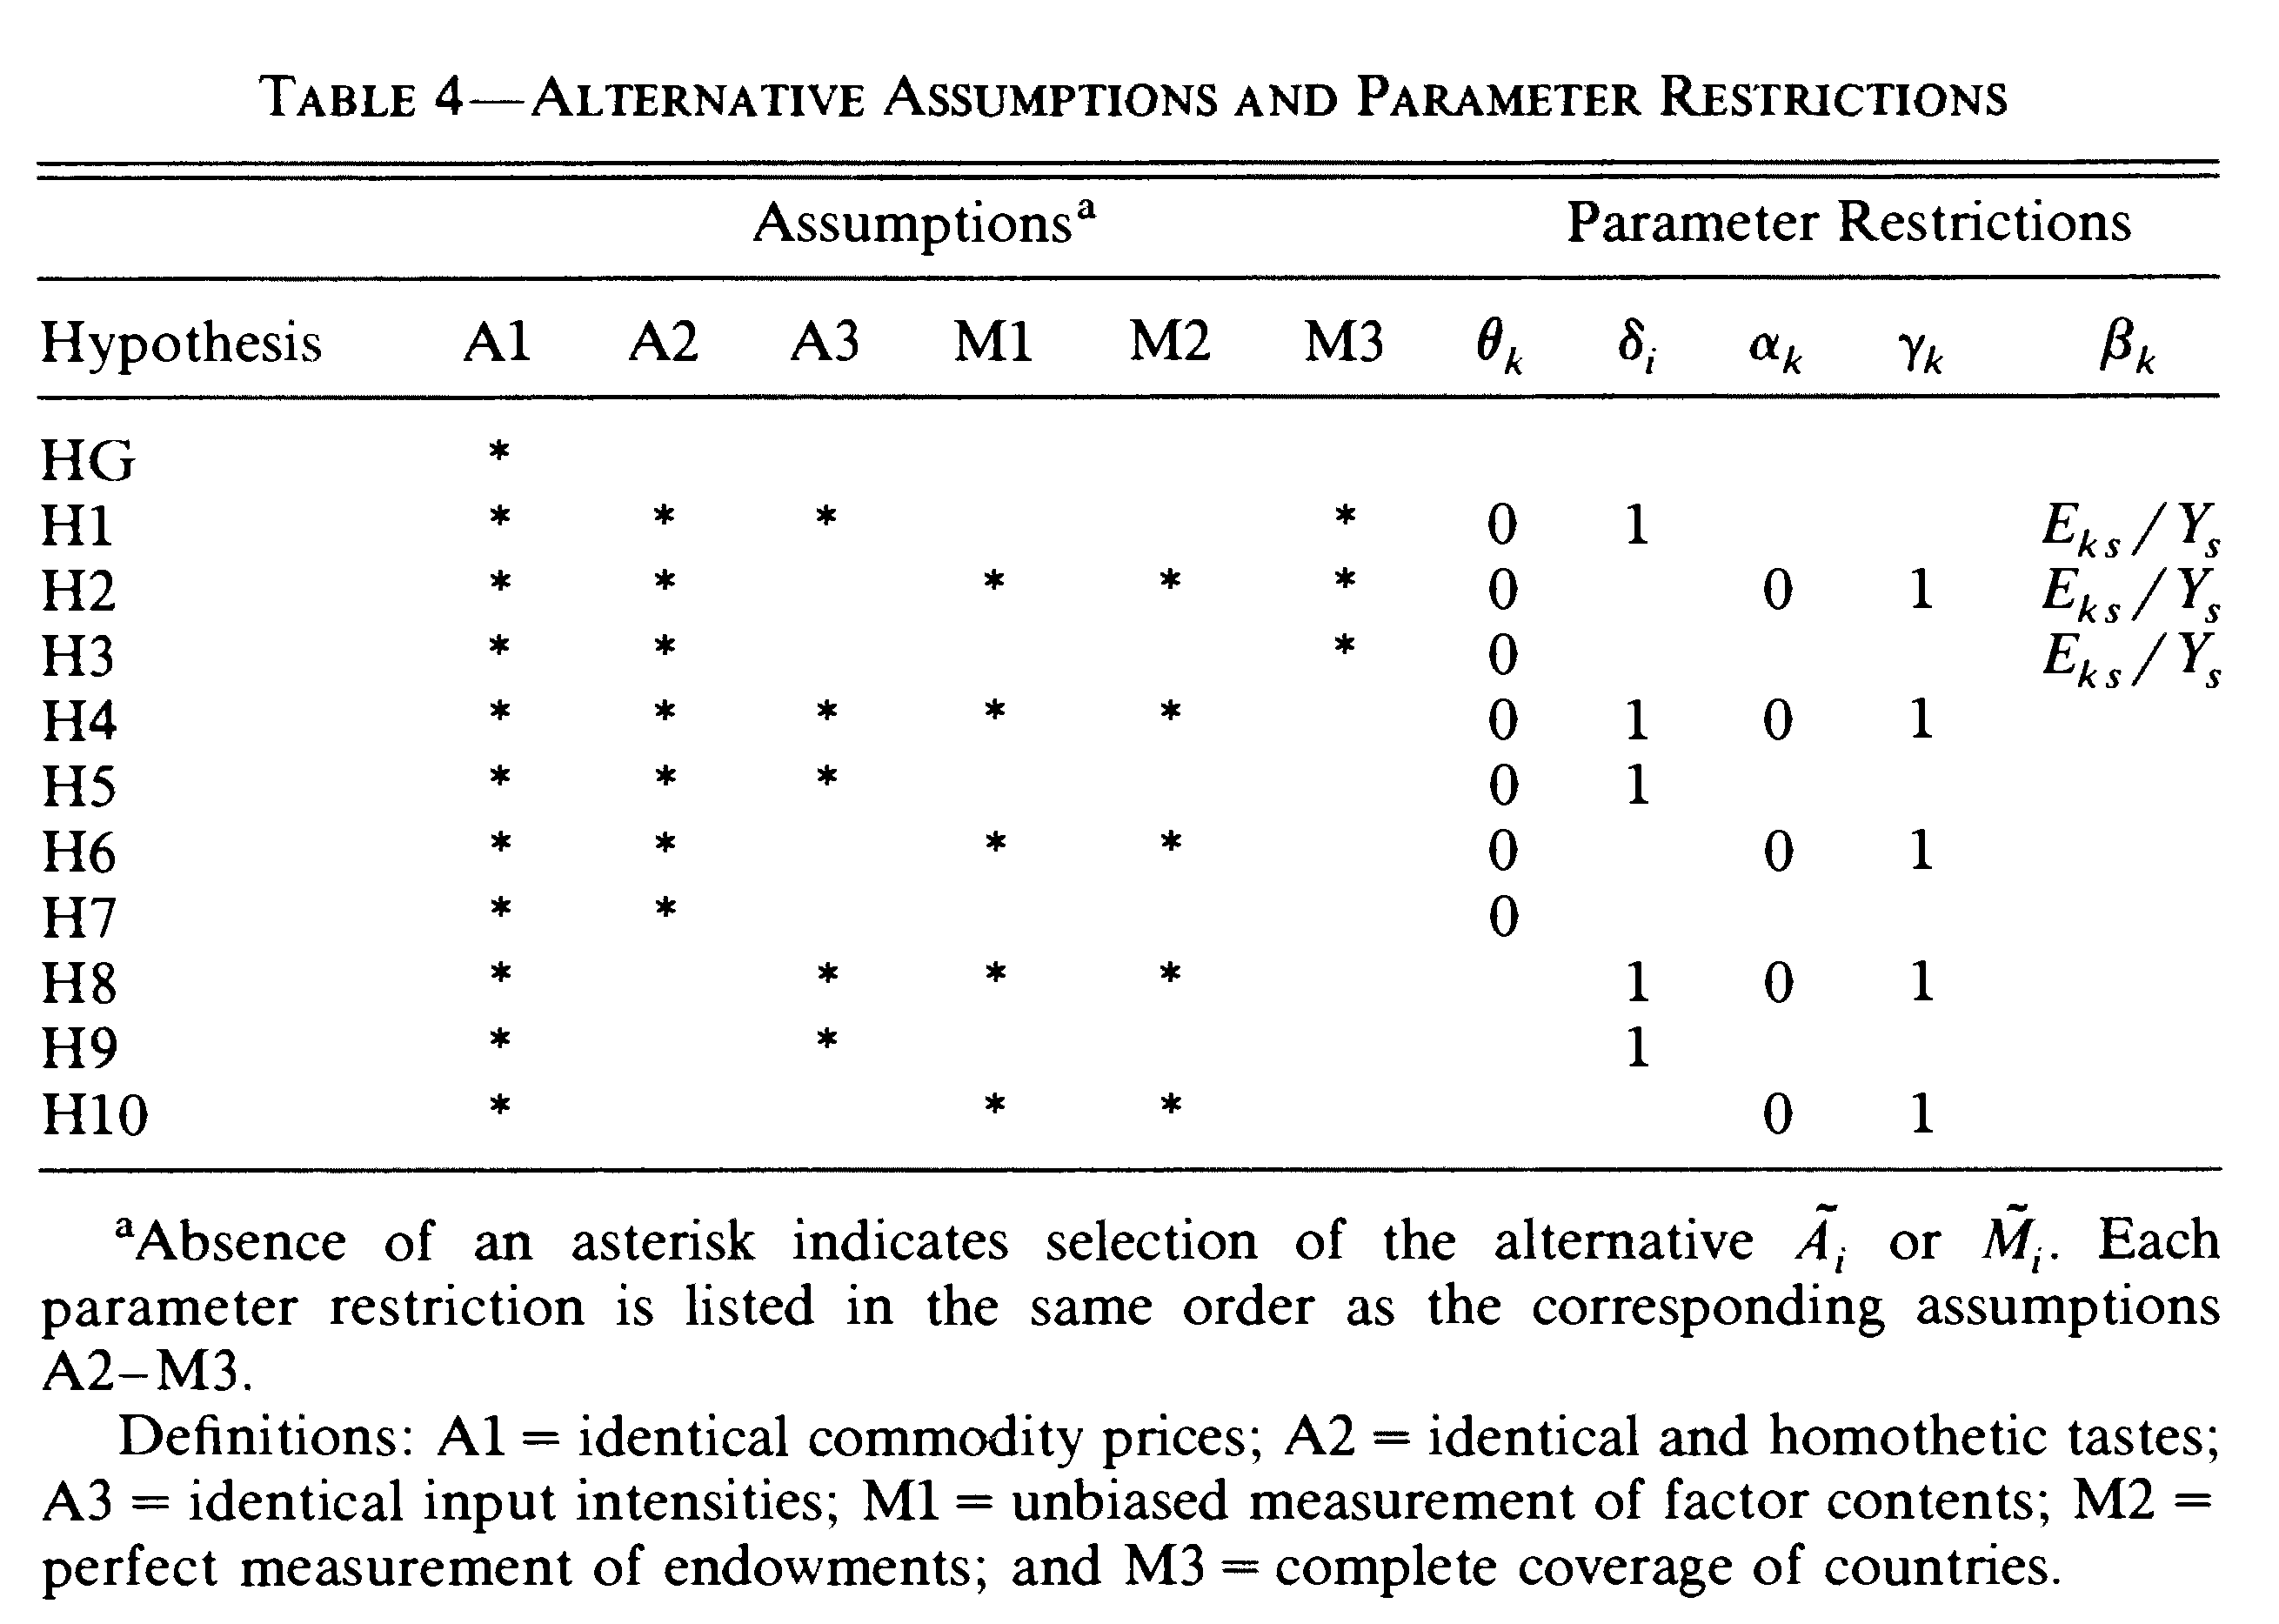
\includegraphics[scale = 0.75]{Table 4.png}
    \label{fig:Table4}
\end{figure} 
    
\end{frame}

%---------------------------------------------------------------

\subsection{Measuring Performance and Estimation Issues}

%---------------------------------------------------------------

\begin{frame}{Likelihood Functions}

\begin{itemize}
    \item<1-> In order to compare the performance of alternative models, we estimate the likelihood function associated with (\ref{eq:generalregressionmodel}):
    \begin{equation*}
        L = \left( ESS \right)^{-NK / 2}
    \end{equation*}
    where $ ESS $ is the error sum of squares summed across countries and factors and $ NK $ is the total number of observations.
    \item<2-> Because $ L $ necessarily increases as we add more parameters, we adjust using the asymptotic Bayes’ formula proposed in Leamer (1978) and Schwarz (1978):
    \begin{equation*}
        L^{*} = L\left( NK \right)^{-p / 2}
    \end{equation*}
    where $ p $ is the number of parameters estimated under a given hypothesis.
\end{itemize}
    
\end{frame}

%---------------------------------------------------------------

\begin{frame}{Likelihood Ratios}

\begin{itemize}
    \item<1-> Given an alternative hypothesis $ j $ and a null hypothesis $ i $, calculate the likelihood ratio:
    \begin{equation*}
        \Lambda = L_{j}^{*} / L_{i}^{*} = \left( \frac{ESS_i}{ESS_j} \right)^{\left( NK / 2 \right)}\left( NK \right)^{\left( p_i - p_j \right)/2}
    \end{equation*}
    The evidence favors hypothesis $ j $ if $ \Lambda > 1 $.
    \item<2-> In order to eliminate heteroskedasticity and scale the variables so that the error terms can be assumed to have the same variance, we scale all variables by the “world” endowment level $ V_{k,s} $ and the country consumption level $ \left( Y_i - B_i \right) $ so that the regression becomes:
    \begin{equation}
        F_{k,i}^{US}S_{k,i} = \alpha_{k}S_{k,i} + \left( \delta_{i} \gamma_{k} \right)\left( V_{k,i}S_{k,i} \right) - \theta_{k}\left( L_{i}S_{k,i} \right) - \frac{\beta_{k}}{V_{k,S}} + F_{k,i}^{e^*}
        \label{eq:modifiedequation3}
    \end{equation}
    where $ S_{k,i} = \left[ \left( Y_i - B_i \right) V_{k,S} \right]^{-1} $ and $ F_{k,i}^{e^*} $ is assumed to be a normally distributed error term.
\end{itemize}
    
\end{frame}

%---------------------------------------------------------------

\begin{frame}{Estimation}

Equation (\ref{eq:modifiedequation3}) is estimated iteratively.

\begin{itemize}
    \item<1-> First $ \delta_i $ (the country fixed effect) is given a seed-value of 1, and the parameters $ \alpha_k $, $ \gamma_k $, $ \theta_k $, and $ \beta_k $ (all factor-specific parameters) are estimated.
    \item<2-> These estimates are then plugged back in to equation (\ref{eq:modifiedequation3}), and $ \delta_i $ is estimated.
    \item<3-> The estimation procedure continues until the likelihood function converges to a stable value.
\end{itemize}
    
\end{frame}

%---------------------------------------------------------------

\subsection{Analysis}

%---------------------------------------------------------------

\begin{frame}{Likelihood Ratio Results}

Table 5 shows the performance of each hypothesis.

\begin{itemize}
    \item<1-> The least restrictive hypothesis (HG) has the lowest ESS value.
    \item<2-> However, the adjusted ESS value is lowest for hypothesis (H3), which allows for proportional changes in technology, biased measurements of the factor content of trade, and mulitiplicative errors in factor endowments, while maintaining homothetic preferences and no sample selection for country coverage.
    \item<3-> The 2nd best is (H7), which is the same as (H3) except allowing for sample selection in country coverage.
    \item<4-> The 3rd best is (HG), the least restrictive sample.  The others are essentially ``impossible" given the data evidence.
\end{itemize}
    
\end{frame}

%---------------------------------------------------------------

\begin{frame}{Table 5}

\begin{figure}
    \centering
    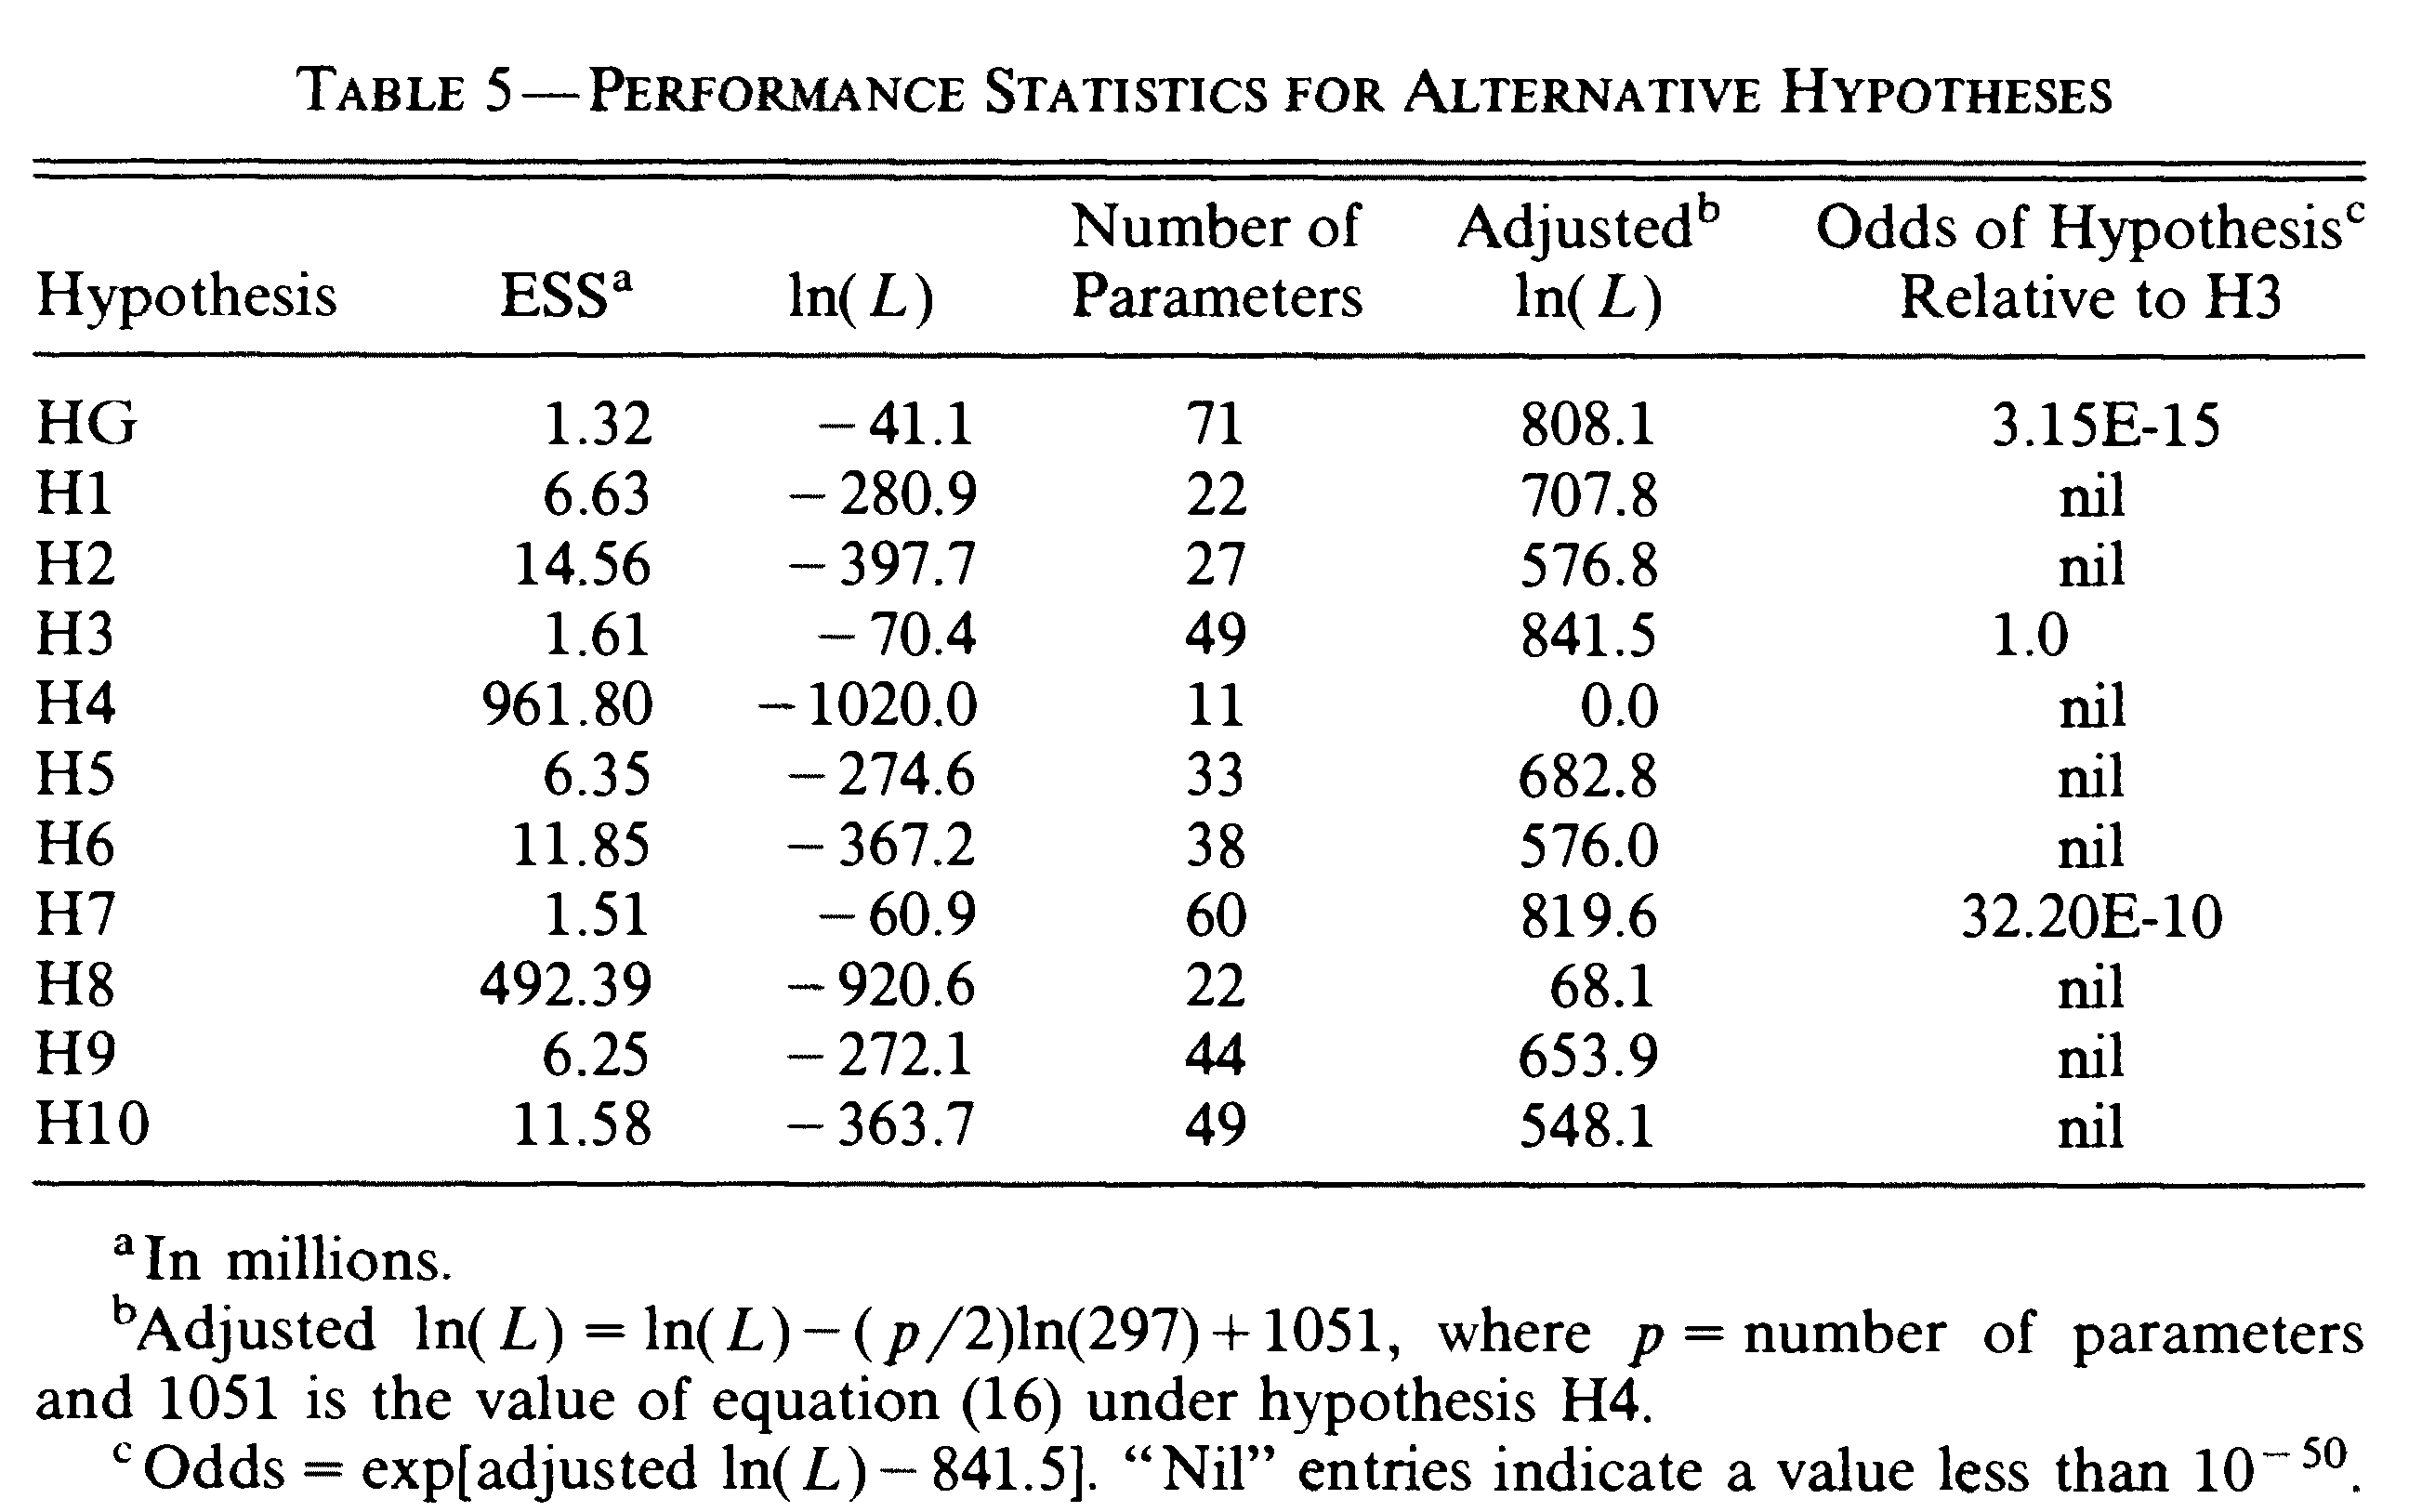
\includegraphics[scale = 1]{Table 5.png}
    \label{fig:Table5}
\end{figure} 
    
\end{frame}

%---------------------------------------------------------------

\begin{frame}{Estimates of $ \delta_i $}

Even though (H3) is the most plausible model, some of its estimates produce implausible values.  Table 6 reports estimates of $ \delta_i $.  8 of 26 countries have impossible negative values, and 15 of 26 have values that are significantly greater than 1, which is unlikely.

\begin{figure}
    \centering
    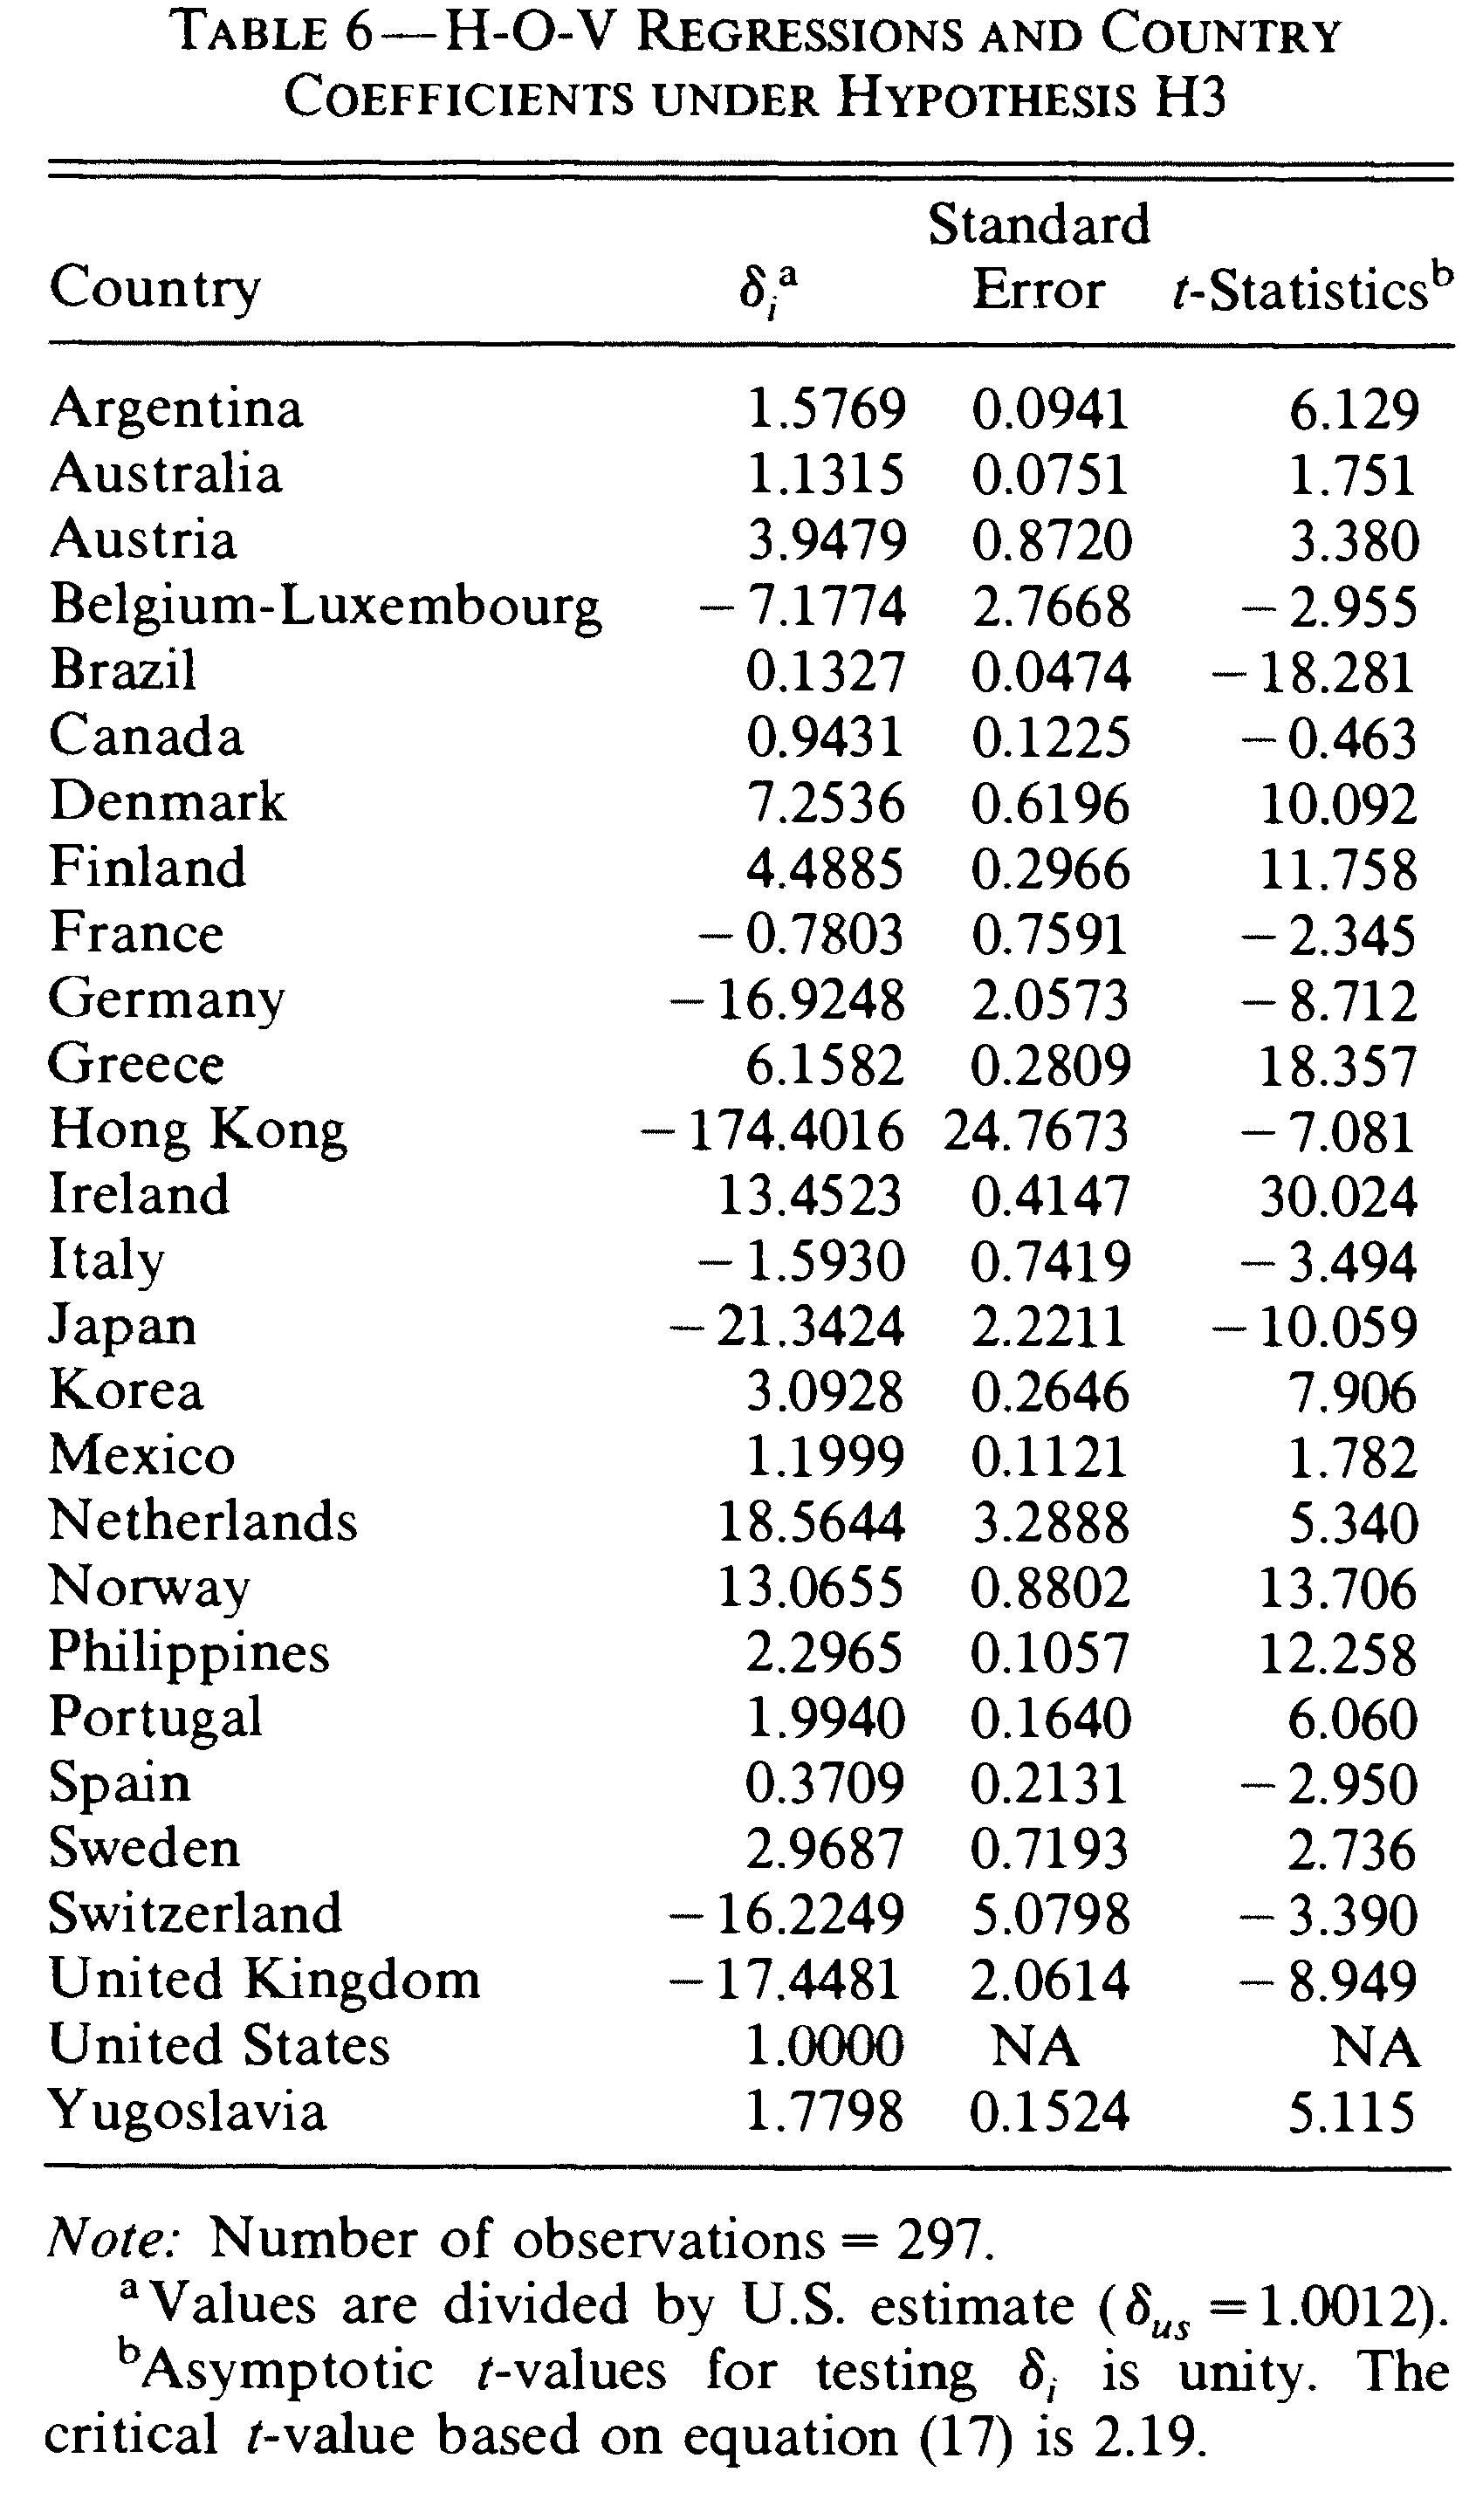
\includegraphics[scale = 0.45]{Table 6.png}
    \label{fig:Table6}
\end{figure} 
    
\end{frame}

%---------------------------------------------------------------

\begin{frame}{Estimates of $ \alpha_k $ and $ \gamma_k $}

Table 7 reports the estimates for the measurement error parameter estimates.  We have no a priori thoughts on the value of $ \alpha_k $, but 4 of the the $ \gamma_k $ coefficient estimates are negative, implying that the observed factor endowments are negatively correlated with the true factor endowments.

\begin{figure}
    \centering
    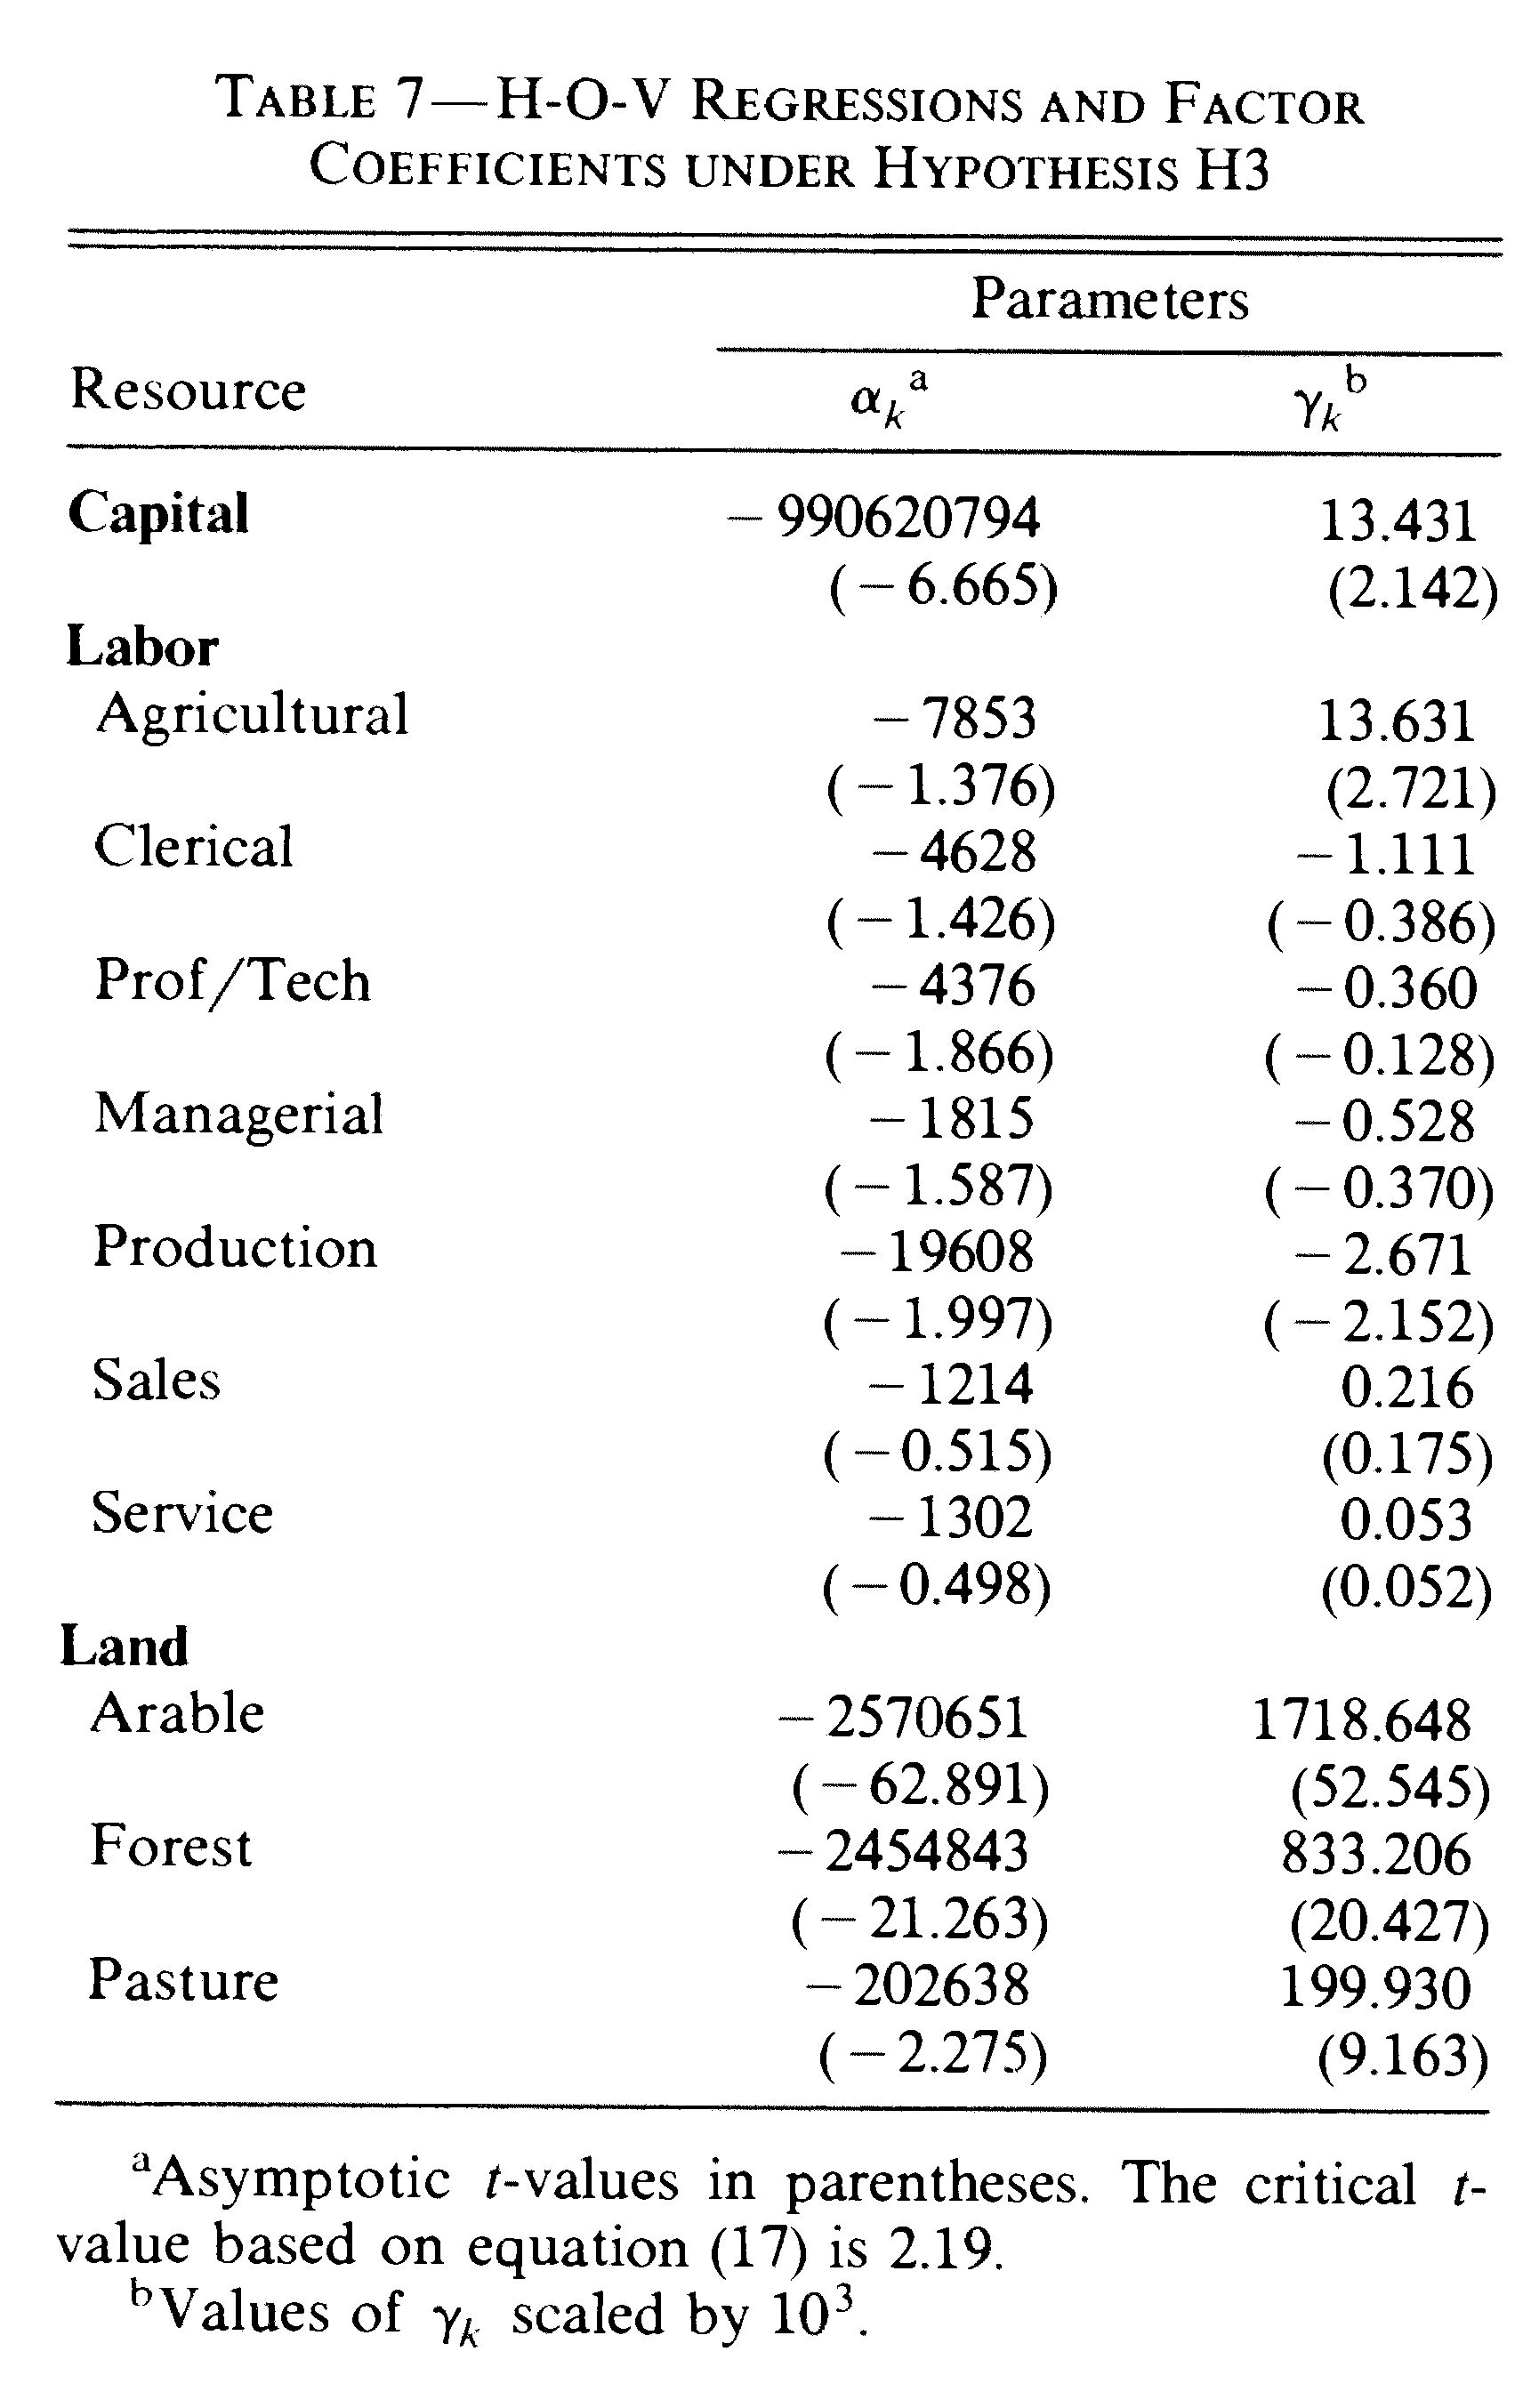
\includegraphics[scale = 0.45]{Table 7.png}
    \label{fig:Table7}
\end{figure} 
    
\end{frame}

%---------------------------------------------------------------

\end{document}